% % % % % % % % % % % % % % % % % % % % % % % % % % % % % % % % % %
\documentclass[runningheads]{llncs}

\newcommand{\project}{{\sc MetaSpy}\xspace}

% packages
\usepackage{xspace}
\usepackage{ifthen}
\usepackage{amsbsy}
\usepackage{amssymb}
\usepackage{balance}
\usepackage{booktabs}
\usepackage{graphicx}
\usepackage{multirow}
\usepackage{needspace}
\usepackage{microtype}
\usepackage{bold-extra}

% constants
\newcommand{\Title}{Domain-Specific Profiling}
\newcommand{\TitleShort}{\Title}
\newcommand{\Authors}{Alexandre Bergel$^1$, Lukas Renggli, Jorge Ressia$^2$}
\newcommand{\AuthorsShort}{A. Bergel, L. Renggli, J. Ressia}

% references
\usepackage[colorlinks]{hyperref}
\usepackage[all]{hypcap}
\setcounter{tocdepth}{2}
\hypersetup{
	colorlinks=true,
	urlcolor=black,
	linkcolor=black,
	citecolor=black,
	plainpages=false,
	bookmarksopen=true,
	pdfauthor={\Authors},
	pdftitle={\Title}}

\def\chapterautorefname{Chapter}
\def\appendixautorefname{Appendix}
\def\sectionautorefname{Section}
\def\subsectionautorefname{Section}
\def\figureautorefname{Figure}
\def\tableautorefname{Table}
\def\listingautorefname{Listing}

% source code
\usepackage{xcolor}
\usepackage{textcomp}
\usepackage{listings}
\definecolor{source}{gray}{0.9}
\lstset{
	language={},
	% characters
	tabsize=3,
	upquote=true,
	escapechar={!},
	keepspaces=true,
	breaklines=true,
	alsoletter={\#:},
	breakautoindent=true,
	columns=fullflexible,
	showstringspaces=false,
	basicstyle=\footnotesize\sffamily,
	% background
	frame=single,
    framerule=0pt,
	backgroundcolor=\color{source},
	% numbering
	numbersep=5pt,
	numberstyle=\tiny,
	numberfirstline=true,
	% captioning
	captionpos=b,
	% formatting (html)
	moredelim=[is][\textbf]{<b>}{</b>},
	moredelim=[is][\textit]{<i>}{</i>},
	moredelim=[is][\color{red}\uwave]{<u>}{</u>},
	moredelim=[is][\color{red}\sout]{<del>}{</del>},
	moredelim=[is][\color{blue}\underline]{<ins>}{</ins>}}
\newcommand{\ct}{\lstinline[backgroundcolor=\color{white},basicstyle=\footnotesize\ttfamily]}
\newcommand{\lct}[1]{{\small\tt #1}}

% tikz
% \usepackage{tikz}
% \usetikzlibrary{matrix}
% \usetikzlibrary{arrows}
% \usetikzlibrary{external}
% \usetikzlibrary{positioning}
% \usetikzlibrary{shapes.multipart}
% 
% \tikzset{
% 	every picture/.style={semithick},
% 	every text node part/.style={align=center}}

% proof-reading
\usepackage{xcolor}
\usepackage[normalem]{ulem}
\newcommand{\ra}{$\rightarrow$}
\newcommand{\ugh}[1]{\textcolor{red}{\uwave{#1}}} % please rephrase
\newcommand{\ins}[1]{\textcolor{blue}{\uline{#1}}} % please insert
\newcommand{\del}[1]{\textcolor{red}{\sout{#1}}} % please delete
\newcommand{\chg}[2]{\textcolor{red}{\sout{#1}}{\ra}\textcolor{blue}{\uline{#2}}} % please change
\newcommand{\chk}[1]{\textcolor{ForestGreen}{#1}} % changed, please check

% comments \nb{label}{color}{text}
\newboolean{showcomments}
\setboolean{showcomments}{true}
\ifthenelse{\boolean{showcomments}}
	{\newcommand{\nb}[3]{
		{\colorbox{#2}{\bfseries\sffamily\scriptsize\textcolor{white}{#1}}}
		{\textcolor{#2}{\sf\small$\blacktriangleright$\textit{#3}$\blacktriangleleft$}}}
	 \newcommand{\version}{\emph{\scriptsize$-$Id$-$}}}
	{\newcommand{\nb}[2]{}
	 \newcommand{\version}{}}
\newcommand{\rev}[2]{\nb{Reviewer #1}{red}{#2}}
\newcommand{\ab}[1]{\nb{Alexandre}{blue}{#1}}
\newcommand{\lr}[1]{\nb{Lukas}{orange}{#1}}
\newcommand{\jr}[1]{\nb{Lukas}{green}{#1}}

% graphics: \fig{position}{percentage-width}{filename}{caption}
\DeclareGraphicsExtensions{.png,.jpg,.pdf,.eps,.gif}
\graphicspath{{figures/}}
\newcommand{\fig}[4]{
	\begin{figure}[#1]
		\centering
		\includegraphics[width=#2\textwidth]{#3}
		\caption{\label{fig:#3}#4}
	\end{figure}}

% abbreviations
\newcommand{\ie}{\emph{i.e.,}\xspace}
\newcommand{\eg}{\emph{e.g.,}\xspace}
\newcommand{\etc}{\emph{etc.}\xspace}
\newcommand{\etal}{\emph{et al.}\xspace}

% lists
\newenvironment{bullets}[0]
	{\begin{itemize}}
	{\end{itemize}}

\newcommand{\seclabel}[1]{\label{sec:#1}}


% D O C U M E N T
% % % % % % % % % % % % % % % % % % % % % % % % % % % % % % % % % %
\begin{document}

% T I T L E
% % % % % % % % % % % % % % % % % % % % % % % % % % % % % % % % % %

\title{\Title}
\titlerunning{\TitleShort}

\author{\Authors} 
\authorrunning{\AuthorsShort}

\institute{$^1$ PLEIAD Lab, University of Chile, Santiago, Chile\\
	\url{http://pleiad.dcc.uchile.cl} \\[0.3cm]
	$^2$ Software Composition Group, University of Bern, Switzerland\\
	\url{http://scg.unibe.ch}\\[0.3cm]
%	\url{abergel@dcc.uchile.cl}\\
%	\url{renggli@me.com}\\
%	\url{jorge.ressia@gmail.com}
	}

\maketitle

% A B S T R A C T
% % % % % % % % % % % % % % % % % % % % % % % % % % % % % % % % % %

\begin{abstract}
	Domain-specific languages and models are increasingly used within general-purpose host languages. While traditional profiling tools perform well on host language code itself, they often fail to provide meaningful results if the developers start to abstract from traditional source code. In this paper we demonstrate the need of dedicated profiling tools with three different case-studies. Furthermore, we present an infrastructure that enables developers to quickly prototype new profilers for their domain-specific models or languages.
\end{abstract}

% % % % % % % % % % % % % % % % % % % % % % % % % % % % % % % % % %
\section{Introduction}\seclabel{introduction}

Profiling is the recording and analysis of a program execution. Profiling is often considered essential when one wants to obtain the  representation of a program execution.

- Specific domain are very present in today software development

- Whereas research on domain-specific languages made great progresses on language specification, implementation and verification, little has been done on profiling.

- Comparison with previous work on domain-specific code checking \cite{Reng10b}.

- Our approach to profiling \cite{Berg10c}. Our strategy to apply it to specific domains (maybe with figure).

The contributions of this paper are: (1) the identification of the need for domain-specific profilers, (2) the presentation of various real-world case-studies where domain-specific profilers helped to significantly improve performance and correctness of domain-specific code, and (3) the presentation of an infrastructure for prototyping domain-specific profilers.

The remainder of this paper is structured as follows: \autoref{sec:problem} illustrates the problems of using a general-purpose profiler on code building on top of domain-specific language. \autoref{sec:profiler} introduces our approach to domain-specific profiling with three case-studies. \autoref{sec:implementation} presents our infrastructure to implement domain-specific profilers; and \autoref{sec:conclusion} summarizes the paper and discusses future work.

% % % % % % % % % % % % % % % % % % % % % % % % % % % % % % % % % %
\section{Problem}\seclabel{problem}


%:=========
\subsection{Difficulty of profiling a specific domain}

This section illustrates two shortcomings of traditional profiling techniques when applied to a specific domain.\\

\paragraph{CPU time profiling.}
Mondrian\footnote{\url{http://www.moosetechnology.org/tools/mondrian}}~\cite{Meye06a} is an open and agile visualization engine. 
Mondrian uses a graph, made of possibly nested nodes and edges, to describe a visualization. Mondrian is a crucial component which is used in more than a dozen of independent projects. To meet clients performance requirements, Mondrian's authors are paying a great attention to provide fast and scalable rendering. In June 2010 a serious performance issue was identified\footnote{\url{http://bit.ly/g8GjIh}} when visualizing an enriched dependency structural matrix~\cite{Lava09a}. Tracking down the cause of the poor performance was not a trivial task. We first have used MessageTally, the sample-based code profiled provided by Pharo.

Execution sampling approximates the time spent in an application's methods by periodically stopping a program and recording the current set of methods under executions. Such a profiling technique is relatively accurate since it has little impact on the overall execution.
Beside MessageTally, execution sampling has been adopted by almost all mainstream profilers (JProfiler\footnote{\url{http://www.ej-technologies.com}}, YourKit\footnote{\url{http://www.yourkit.com}}, xprof~\cite{Gupt92a}, hprof\footnote{\url{http://java.sun.com/developer/technicalArticles/Programming/HPROF.html}}).

MessageTally produces a textual output of in which method the interpreter spent some time when rendering the visualization. An except of the output is:

\begin{lstlisting}
54.8% {11501ms} MOCanvas>>drawOn: 
  54.8% {11501ms} MORoot(MONode)>>displayOn: 
   30.9% {6485ms} MONode>>displayOn: 
      | 18.1% {3799ms} MOEdge>>displayOn: 
     	...    
      |  8.4% {1763ms} MOEdge>>displayOn: 
      |    | 8.0% {1679ms} MOStraightLineShape>>display:on: 
      |    |  2.6% {546ms} FormCanvas>>line:to:width:color: 
    	...    
   23.4% {4911ms} MOEdge>>displayOn: 	
        ...    
\end{lstlisting}

It essentially says that the virtual machine spent about 54\% of its time in the method \ct{#displayOn:} defined in the class \ct{MORoot}. A root is the unique non-nested node that contains all the nodes of the edges of the visualization. This general profiling information says that rendering nodes and edges consumes a great share of the CPU, but it does not help pinpointing which nodes and edges are culprit of the time taken. Not all the graphical elements equally consume resources.

MessageTally considers a method frame as the unit of the profiling information. Unfortunately, this has little benefit in explaining the cause of the experienced slowdown. An \emph{ad-hoc} solution consists associating for each element the number of time it has been refreshed. We found out that graphical shape properties such as line width, fill color, border color were constantly computed, even though no variation in the model were produced. 
This performance issue has been solved a few days after the complain via a quantification of the \ct{#displayOn:} invocation on each objects and metric computation.
 The information collected by MessageTally was not useful to solve the problem. 

\paragraph{Coverage.}
PetitParser is a parsing framework combining ideas from scannerless parsing, parser combinators, parsing expression grammars and packrat parsers to model grammars and parsers as objects that can be reconfigured dynamically \cite{Reng10c}. %PetitParser is designed to be fast: parsing a textual input is significantly faster than SmaCC, a widely used lalr parser implemented in Pharo.

A number of grammars have been implemented, including Java, Smalltalk, XML and SQL. Grammars written in PetitParser may be large. As any piece of software code, duplication and unnecessary rules frequently appear in grammars. Getting the coverage of a grammar for a set of referential input text is useful to identify unused and duplicated parsing rules. 

Beside the CPU consumption, sample-based profiling estimates the method coverage of an application: methods present in the call graph are covered by the referential input text. For example, the Java grammar is defined with 210 rules\footnote{\url{http://www.squeaksource.com/PetitJava.html}}.

\ab{Add example}

%:=========
\subsection{Summary of the problem}

Current profilers are useful to gather runtime data (\eg method invocations, method coverage, call trees, memory consumption, \etc) from the static code model offered by the programming language (\eg packages, classes, methods, statements, \etc). This works well for to profile concerns at the abstraction level of the programming language like execution time, invocation count, memory consumption, code coverage, flow analysis, \etc.

In many today's software there is a significant gap between the model offered by the execution platform and the model of the actually running application. The proliferation of meta-models and domain-specific languages builds new abstractions that map to the underlying execution platform in non-trivial ways. Traditional profiling tools fail to display relevant information in the presence of such abstractions.

% % % % % % % % % % % % % % % % % % % % % % % % % % % % % % % % % %

\section{Domain-Specific Profiler}\seclabel{profiler}

%:========
\subsection{Properties of a Domain-Specific Profiler}

\lr{These are the points we are addressing, thus it should go to the problem section. No? And in this section we show how we solve them.}

\paragraph{Domain-Specific Collection.}
 having the profiler aware of elements to be profiled, and not about their implementation. perform profiling on the abstraction of the domain, not in the host language

\paragraph{Domain-Specific Presentation.} Information obtained during a code execution profiling needs to be adequately presented to be exploitable. A graph (composed of nodes and edges) is a structure general enough to describe meta-models.

The profiling information need to be mapped back to the profiled model. This implies that the presentation should provide enough information to be able to navigate between the profile to the model.

\paragraph{Homogeneous event cost.}
When considering the execution time of a particular event, each event must be treated as an atomic and uniform operation, independently of the object receiver. \ab{maybe not... We need to experiment on this} \lr{I don't get it.} \lr{Maybe more ``Domain-Specific Evaluation'', \ie arguing that time-to-run, number of activations, ... does not make sense; we need domain-specific values like characters/second, refreshes/click, ...}

\paragraph{Domain-Specific Evolution.} 
More importance on variation than absolute number. \lr{How does the profile change over time?}

\paragraph{Domain-Specific Scope.} 
Dealing with circularity and meta-references is a common issue when a profiler is an instance of the model being profiled. To keep the model distinct from the profiler, a scoping mechanism has to be employed~\cite{Tant10a}.


%:========
\subsection{The \project Framework}

\fig{}{.8}{MetaSpy}{The \project framework.}


\project is a framework to easily build domain specific profiler. 

\begin{tabular}{c|c|c}
					&	\textbf{Host language} 	& \textbf{DSL} \\ \hline
					&						& 		\\
\textbf{$M_0$ - Static}	&	classes, methods		& 		\\
					&						& 		\\\hline
					&						& Mondrian\\
\textbf{$M_1$ - Dynamic}	&	method activation		& OB-metamodel\\
					&						& Grammars\\ \hline
					&						& OB Browser\\
\textbf{$M_2$ -} 		&						& Visualization\\
					&						& Mondrian
\end{tabular}


%:========
\subsection{Case Study: Caches in Mondrian}


To meet clients performance requirements, Mondrian comprises a number of intertwined cache mechanisms. We applied \project to profile the activation of caches in Mondrian.

\paragraph{Keeping track of the caches activations.}
Each nodes has a number of caches. Activation of theses caches are under complex rules which depends on what is currently displayed, the nesting of nodes and their size. An improper implementation of the caches are a source of hard-to-track bugs and abnormal behavior.

The following code excerpt monitors the cache activation in a Mondrian easel.

\begin{lstlisting}[numbers=left]
| view allNodes |
view := MOViewRenderer new.
view interaction every: 1500 do: [
	view root clear.
	view shape rectangle
		<b>if: #hasCachedForm fillColor: Color red</b>.
	allNodes := <b>easel canvas root allNodes</b>.
	view nodes: allNodes forEach: [:each |
		<b>view nodes: each metricCaches</b>.
		view gridLayout gapSize: 2.
	].  
	<b>view edges: allNodes from: #owner to: #yourself</b>.
	view treeLayout.
	view root applyLayout. ].	
view open.
\end{lstlisting}

The code opens a new Mondrian visualization that visualizes the rendering of the visualization given in an easel. The \emph{domain} that is profiled are the node obtained from the easel. Lines 7 and 12 shows this: nodes are acquired from the easel and the ownership is represented with edges. The \emph{domain is profiled} against two relevant properties. These are represented in Lines 6 and 9: a bitmap form and metrics may are separately cached. The \emph{profile presentation} is made via a Mondrian script. The \emph{evolution over execution} is realized via a periodical refresh, indicated in the script at Line 3. The model being profiled and the profiler are represented with different objects in the host language. The \emph{scope} of the profiling is naturally given by operating on a different object.

\fig{}{.8}{MondrianExample}{Profiling of a Mondrian visualization in Mondrian.}

The profile visualization is given in \autoref{fig:MondrianExample}. The upper part is a visualization example, part of Mondrian tutorial. The below part is a profiling of it. Upper nodes are nesting nodes. The red color indicate that the bitmap form cache is activated, and inner nodes indicates a metric cache. We can see that the fourth red node does not have any metric cache activated. This helped us to fix a number of issues related to the way caches are managed. These issues have been fixed in the Version 6, 9 and 10 of the package Mondrian-Core\footnote{All the versions of Mondrian are available online on \url{http://www.squeaksource.com/Mondrian.html}.}.


\paragraph{Number of display:on:}
A Mondrian visualization may comprise a great deal of graphical elements. At each refresh of the Mondrian visualization dictated by the operating system, only the elements that needs to be refreshed must effectively be. Elements that are outside the window or for which a bitmap form cache is active should not be refreshed. 

A graphical element is refreshed when the method {\sf \#display:on:} is invoked. Monitoring when these invocations occur is key to have a global view of what get refreshed. Such a monitoring is realized via method instrumentation~\cite{Berg10d}. The instrumentation is realized via the method:

\begin{lstlisting}[numbers=left]
MondrianProfilerMethod>>beforeRun: methodName with: listOfArguments in: receiver
	((<b>methodName == #display:on:</b> ) 
		and: [ <b>listOfArguments first model isNumber</b> ])
			ifTrue: 
				[ | v |
				  v := listOfArguments first.
				  counter at: v put: ((counter at: v ifAbsentPut: [ 0 ]) + 1 ) ]
\end{lstlisting}

Line 2 defines the domain of what has to be profiled, invocation of the {\sf \#display:on:} method. The scope of the profiling is restricted to element that are actually numbers, this is what our visualization under profiling is operating on. 

\fig{}{.6}{MondrianProfiler}{Profiling Mondrian.}

\autoref{fig:MondrianProfiler} gives a screenshot of the Mondrian profiler. The right hand side gives a ...


%:========
\subsection{Case Study: Events in Omnibrowser}



\paragraph{Meta-model instantiation}
\begin{lstlisting}
	model := OBSystemBrowser onClass: Object selector: #printOn:.
	profile := OmniProfiler 
		profile: [ window :=  model open ]
		inPackage: 'OmniBrowser'.
\end{lstlisting}

\paragraph{Recording events}
\begin{lstlisting}
	model := OBSystemBrowser onClass: Object.
	actualCounter := Dictionary new.
	previousCounter := Dictionary new.
	model announcer
		observe: OBAnnouncement
		do: [ :ann | actualCounter at: ann class put: (actualCounter at: ann class ifAbsentPut: [ 0 ]) + 1 ].
\end{lstlisting}


%:========
\subsection{Case Study: Parsing Framework with PetitParser}


Rigorous test suites try to ensure that each part of the grammar is covered by tests and well specified according to the respective language standards. Validating that each production of the grammar is covered by the tests is a difficult activity. As mentioned previously, the traditional tools of the host language work on a method- and statement-level and thus cannot produce meaningful results in the context of PetitParser where the grammar is modeled as a graph of objects.

With \project we can implement the grammar coverage with a few lines of code. The instrumentation happens at the level of the primitive parser objects. The method \ct{observeParser:in:} wraps the parser object with a handler block that is called for each activation of the parser.

\begin{lstlisting}[numbers=left]
<b>PetitParserSpy>>setUp</b>
	self grammar allParsers do: [ :parser |
		self observeParser: parser in: self grammar do: [
			counter at: parser put: (counter at: parser ifAbsent: [ 0 ]) + 1 ] ]
\end{lstlisting}

Line~2 iterates over all primitive parser objects in the grammar. Line~3 attaches the event handler on Line~4 to each parser in the model. The handler then counts the activations of each parser object when we run the test suite of the grammar. This provides us with the necessary information to display the grammar coverage in a visualization as seen in \autoref{fig:grammar-coverage}.

\begin{figure}[h!tb]
	\centering
	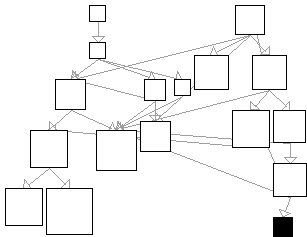
\includegraphics[width=0.4\textwidth]{xml-uncovered}
	\hspace{0.1\textwidth}
	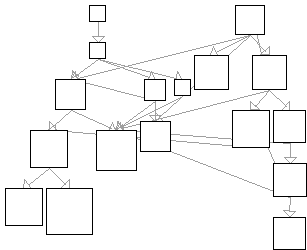
\includegraphics[width=0.4\textwidth]{xml-covered}
	\caption{Production coverage of an XML grammar with uncovered productions highlighted in black (left); and the same XML grammar with updated test coverage and complete production coverage (right). The size of the nodes is proportional to the number of activations when running the test suite on the grammar.}
	\label{fig:grammar-coverage}
\end{figure}

% % % % % % % % % % % % % % % % % % % % % % % % % % % % % % % % % %
\section{Discussion}\seclabel{discussion}

\paragraph{Getting the information.} 
Depend on the application to be profiled. 
Can use events if the application to be profiled has been accordingly designed. This is the case of Omnibrowser. 

Can use bytecode instrumentation. But in that case, high level representation needs to be extracted by the programmer. A mapping has to be explicit. This is the case of PetitParser and Mondrian.




% % % % % % % % % % % % % % % % % % % % % % % % % % % % % % % % % %
\section{Implementation}\seclabel{implementation}

Implemented with the MetaSpy profiling framework

%:========
\subsection{Benchmark}	
	
% % % % % % % % % % % % % % % % % % % % % % % % % % % % % % % % % %
\section{Conclusion}\seclabel{conclusion}

This problem is rather well generalized. For example, profiling a virtual machine is a particularly difficult activity, since instead of providing information about bytecode and primitive executions, the virtual machine talks about functions executions\footnote{\url{http://www.mirandabanda.org/cogblog/2008/12/30/the-idee-fixe-and-the-perfected-profiler/}}.

% % % % % % % % % % % % % % % % % % % % % % % % % % % % % % % % % %
\section*{Acknowledgments}

\small We gratefully thanks ...

% bibliography
% % % % % % % % % % % % % % % % % % % % % % % % % % % % % % % % %
\bibliographystyle{splncs}
\bibliography{scg}

\end{document}